\section{Результаты работы и снимки экрана приложения}
\label{sec:results}

Для подтверждения корректности работы разработанного веб-сервера и взаимодействия с СУБД PostgreSQL было проведено комплексное тестирование всех реализованных сценариев.

Снимок экрана страницы просмотра таблиц схемы представлен на рисунке~\ref{fig:fig-tables}.

\begin{figure}[H]
    \centering
    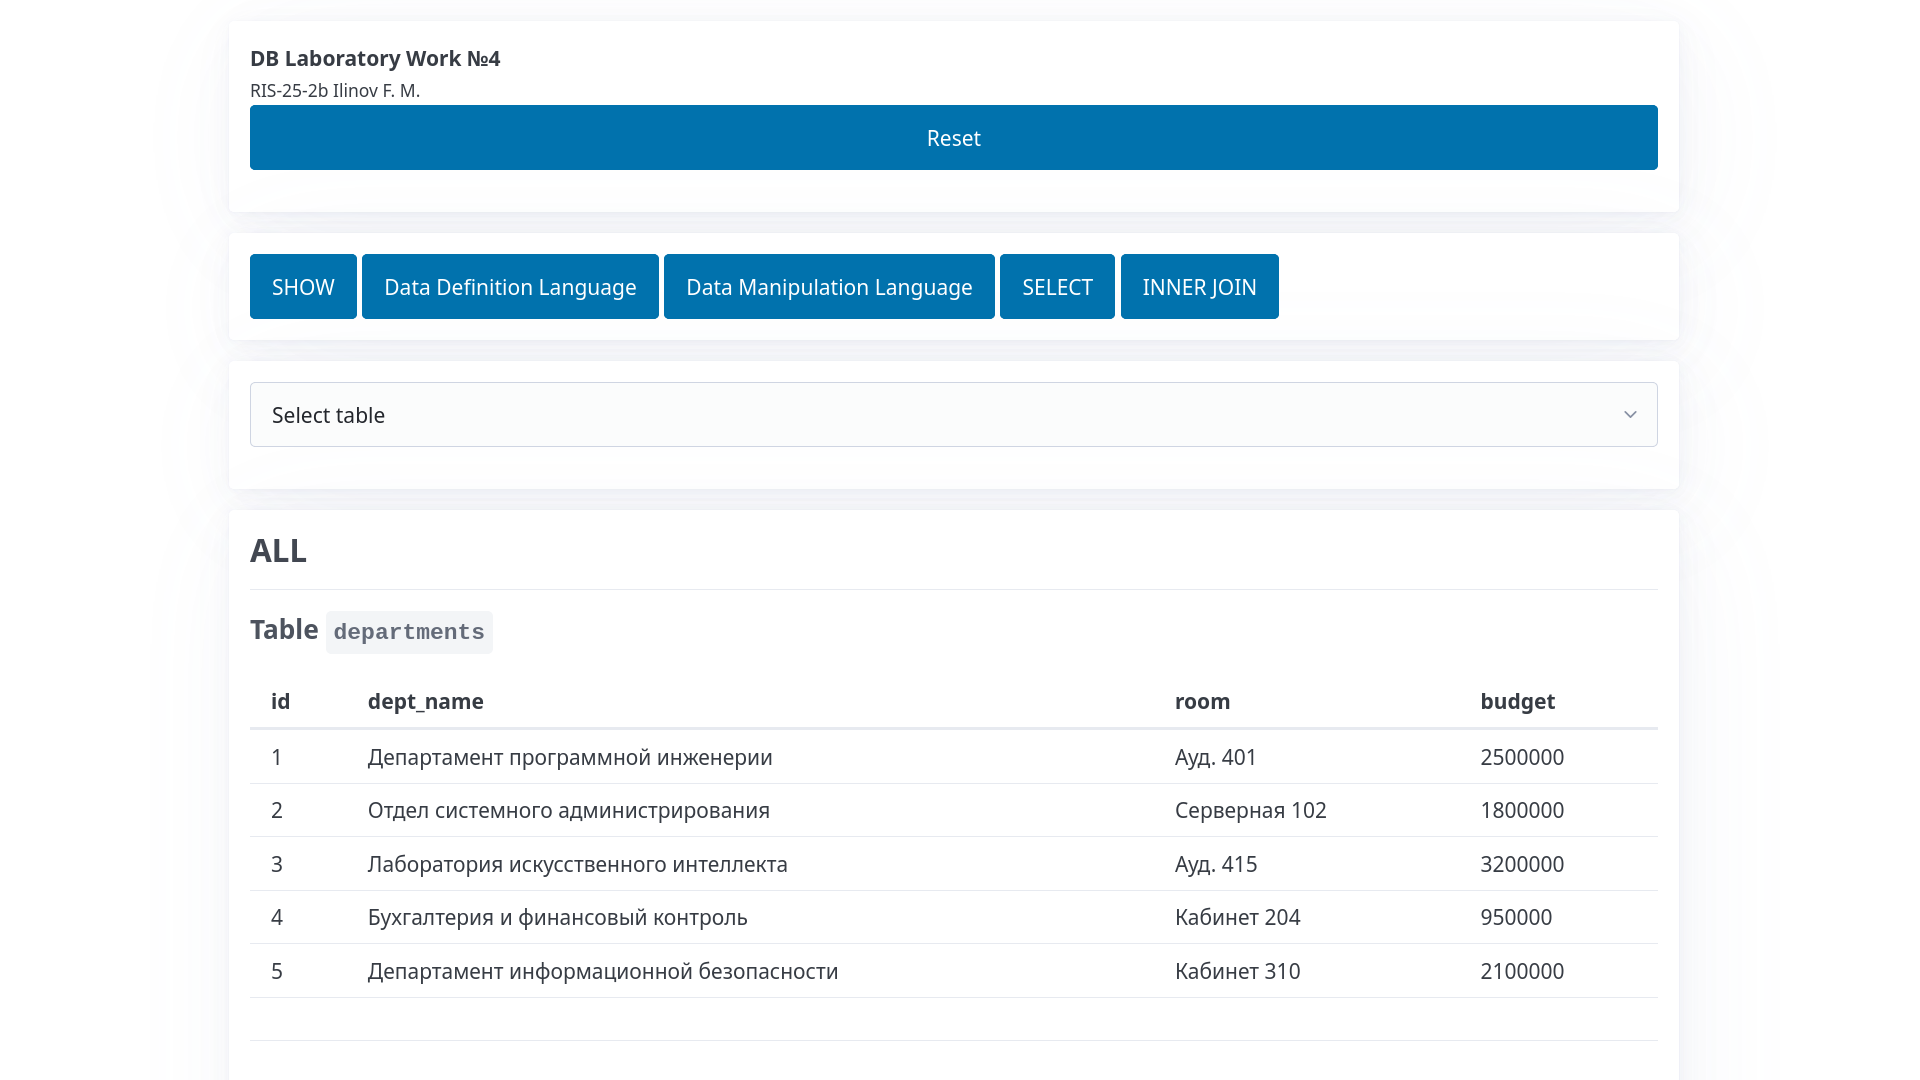
\includegraphics[width=\textwidth]{img_tables}
    \caption{Отображение списка таблиц и их кортежей в браузере}
    \label{fig:fig-tables}
\end{figure}

Снимок экрана создания новой таблицы с первичным и внешним ключами приведен на рисунке~\ref{fig:fig-ddl-create}.

\begin{figure}[H]
    \centering
    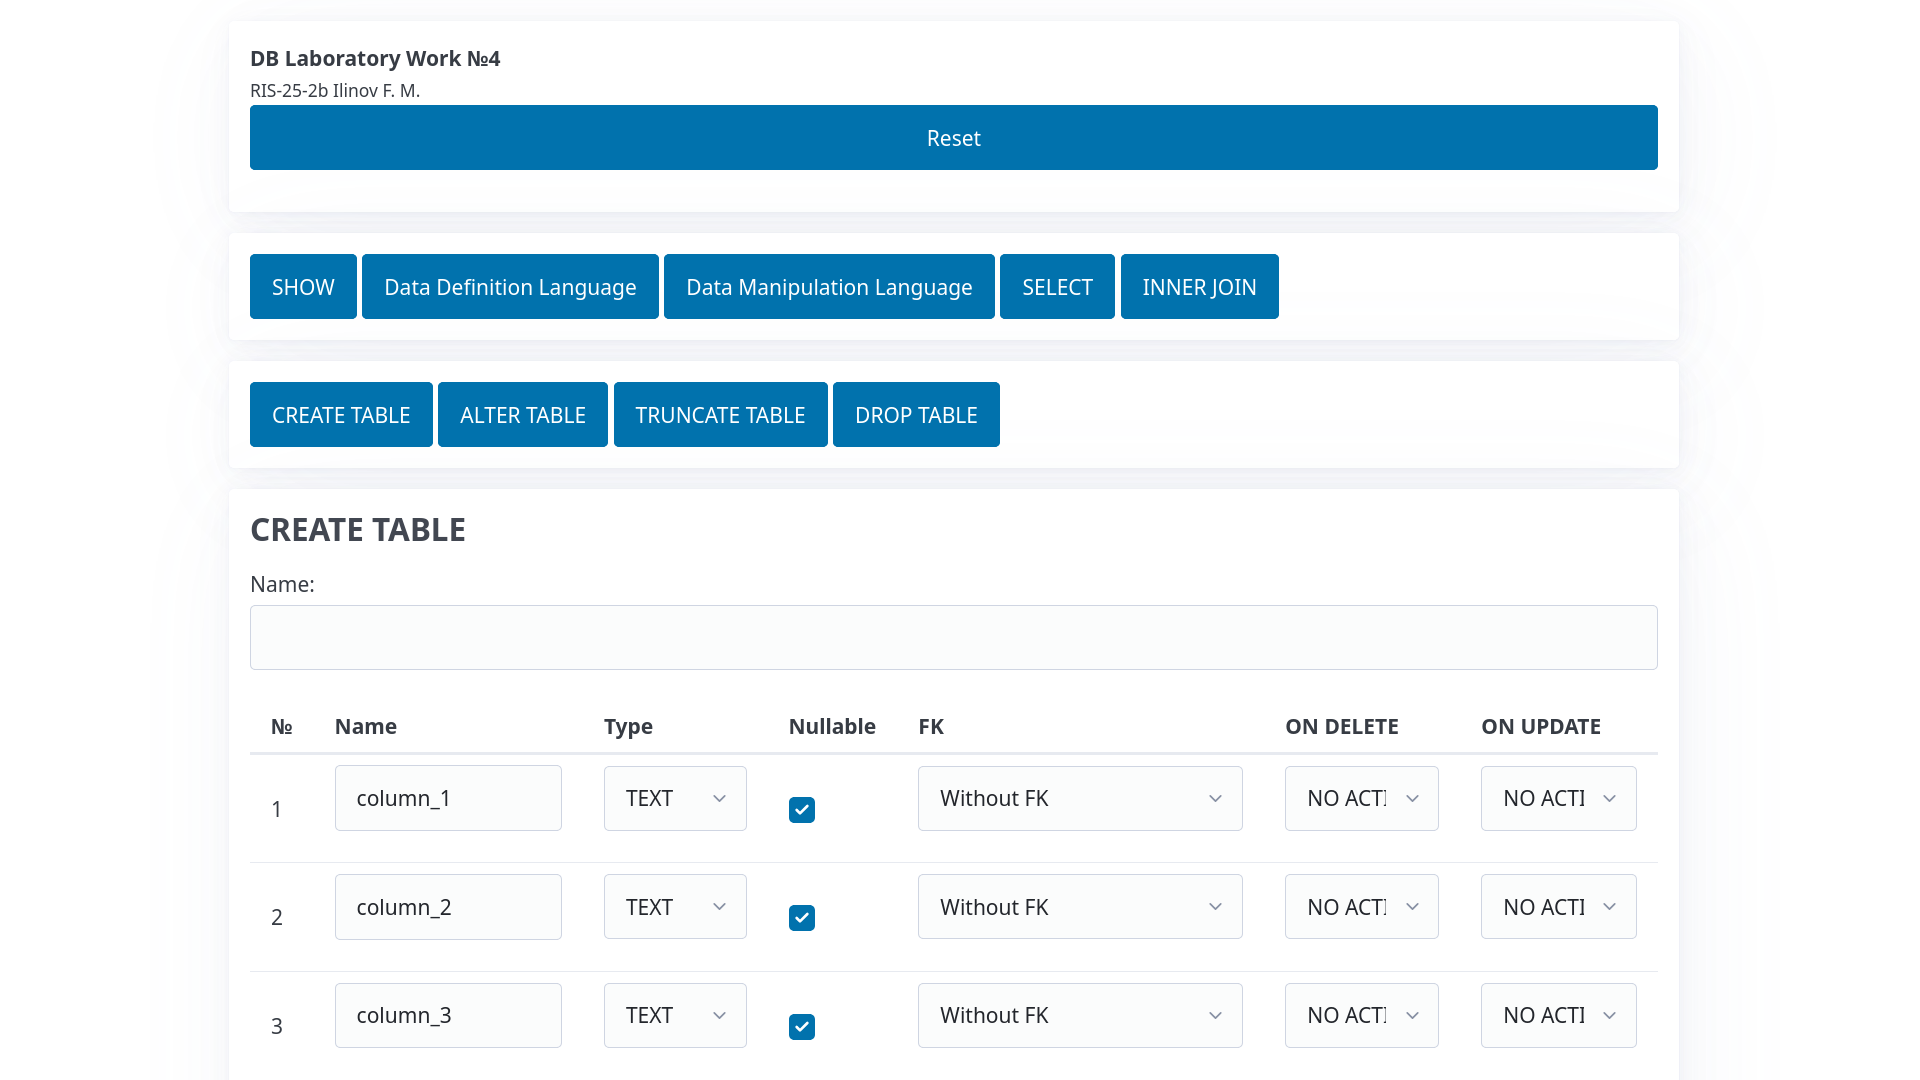
\includegraphics[width=\textwidth]{img_ddl_create}
    \caption{Создание таблицы через двухэтапную форму DDL}
    \label{fig:fig-ddl-create}
\end{figure}

Снимок экрана модификации колонок таблицы с помощью команды ALTER TABLE приведен на рисунке~\ref{fig:fig-ddl-alter}.

\begin{figure}[H]
    \centering
    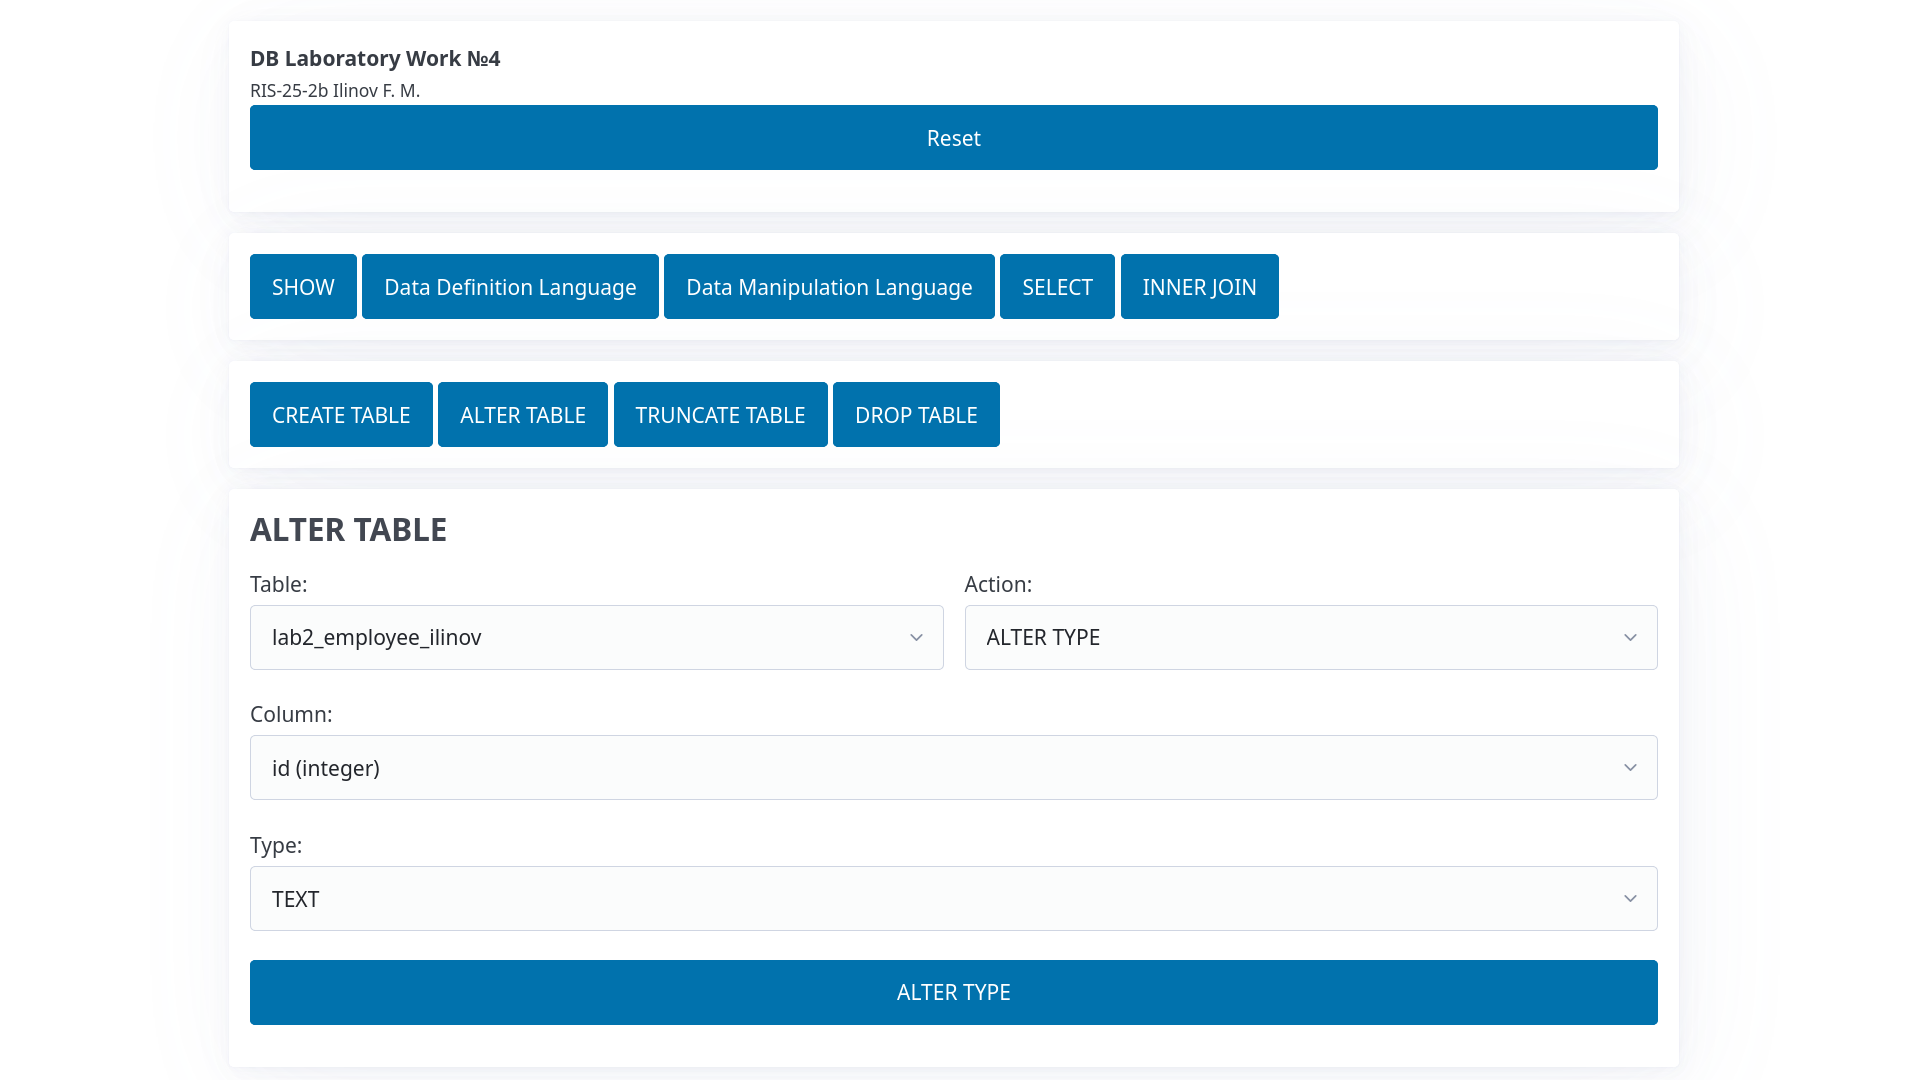
\includegraphics[width=\textwidth]{img_ddl_alter}
    \caption{Модификация структуры таблицы с помощью команды ALTER TABLE}
    \label{fig:fig-ddl-alter}
\end{figure}

Снимок экрана очистки данных таблицы оператором TRUNCATE представлен на рисунке~\ref{fig:fig-ddl-truncate}.

\begin{figure}[H]
    \centering
    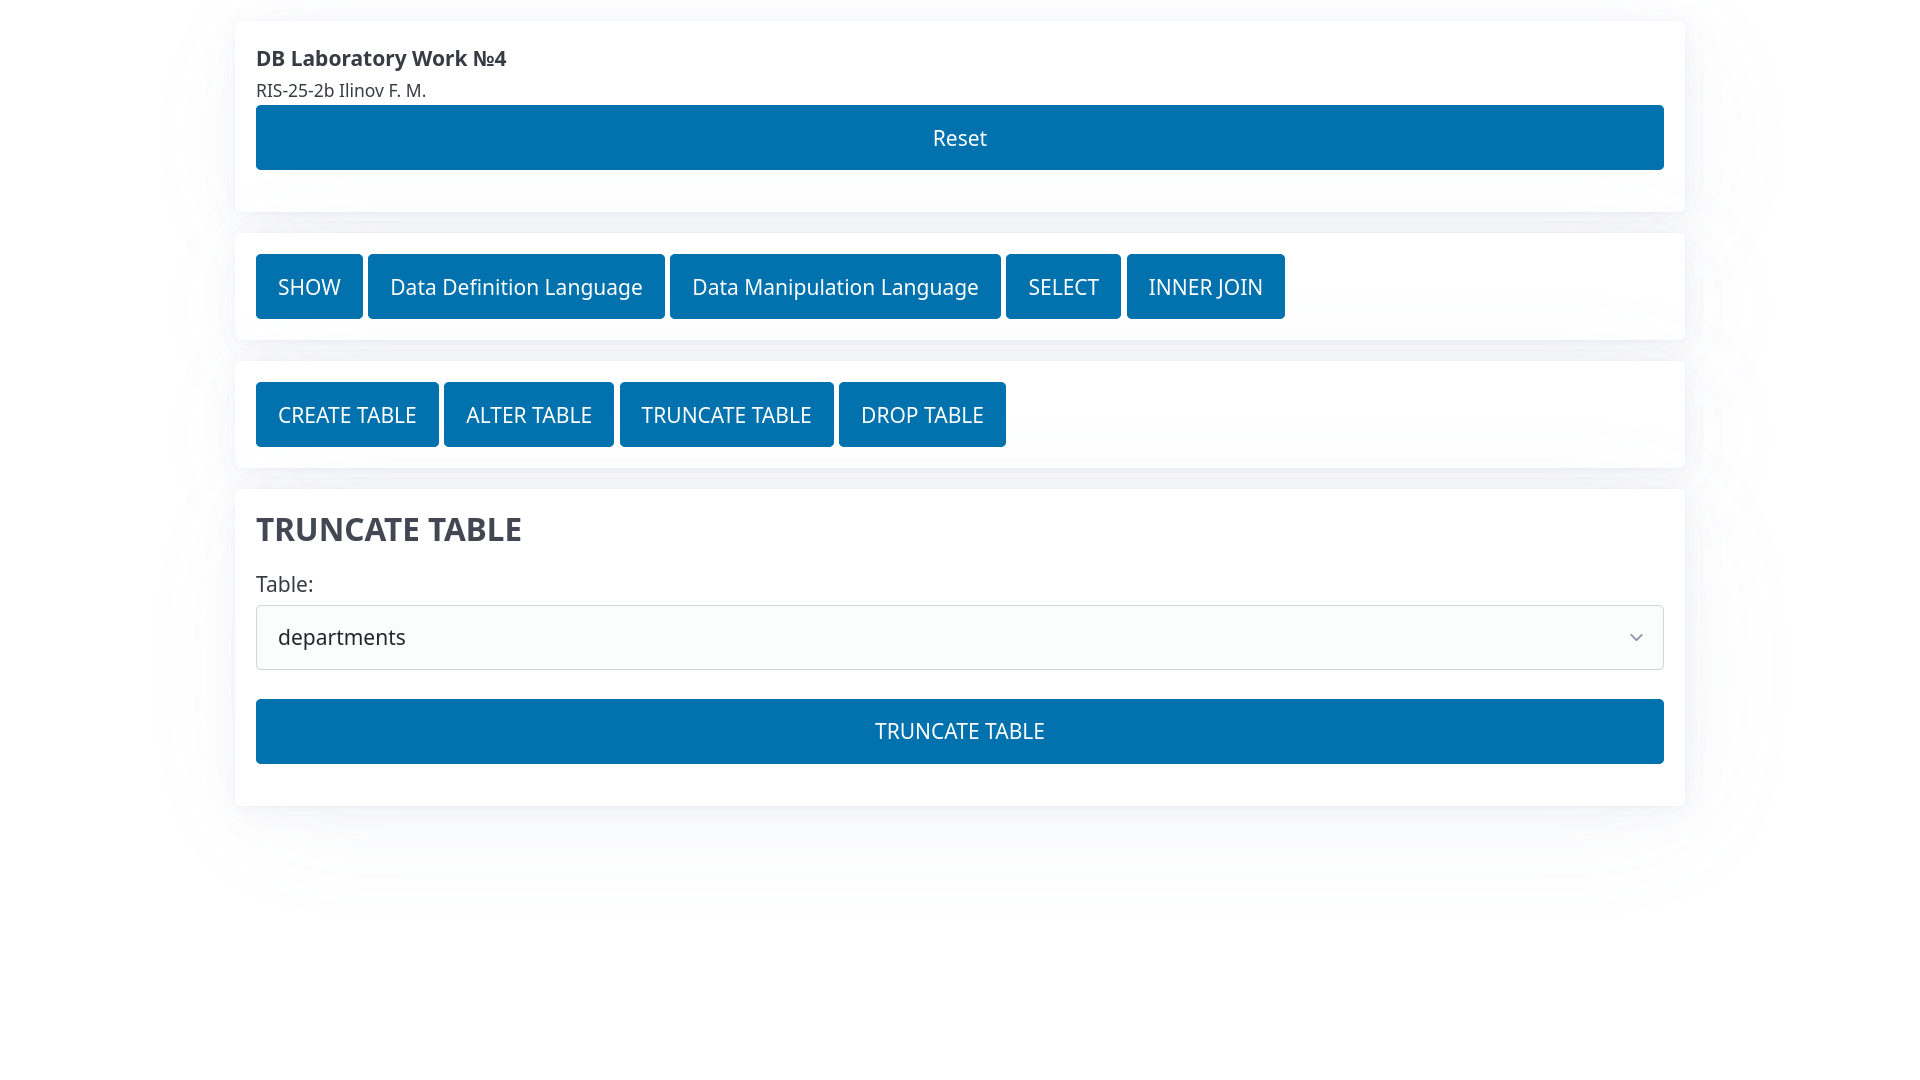
\includegraphics[width=\textwidth]{img_ddl_truncate}
    \caption{Очистка таблицы оператором TRUNCATE TABLE CASCADE}
    \label{fig:fig-ddl-truncate}
\end{figure}

Снимок экрана удаления таблицы с каскадной очисткой связей приведен на рисунке~\ref{fig:fig-ddl-drop}.

\begin{figure}[H]
    \centering
    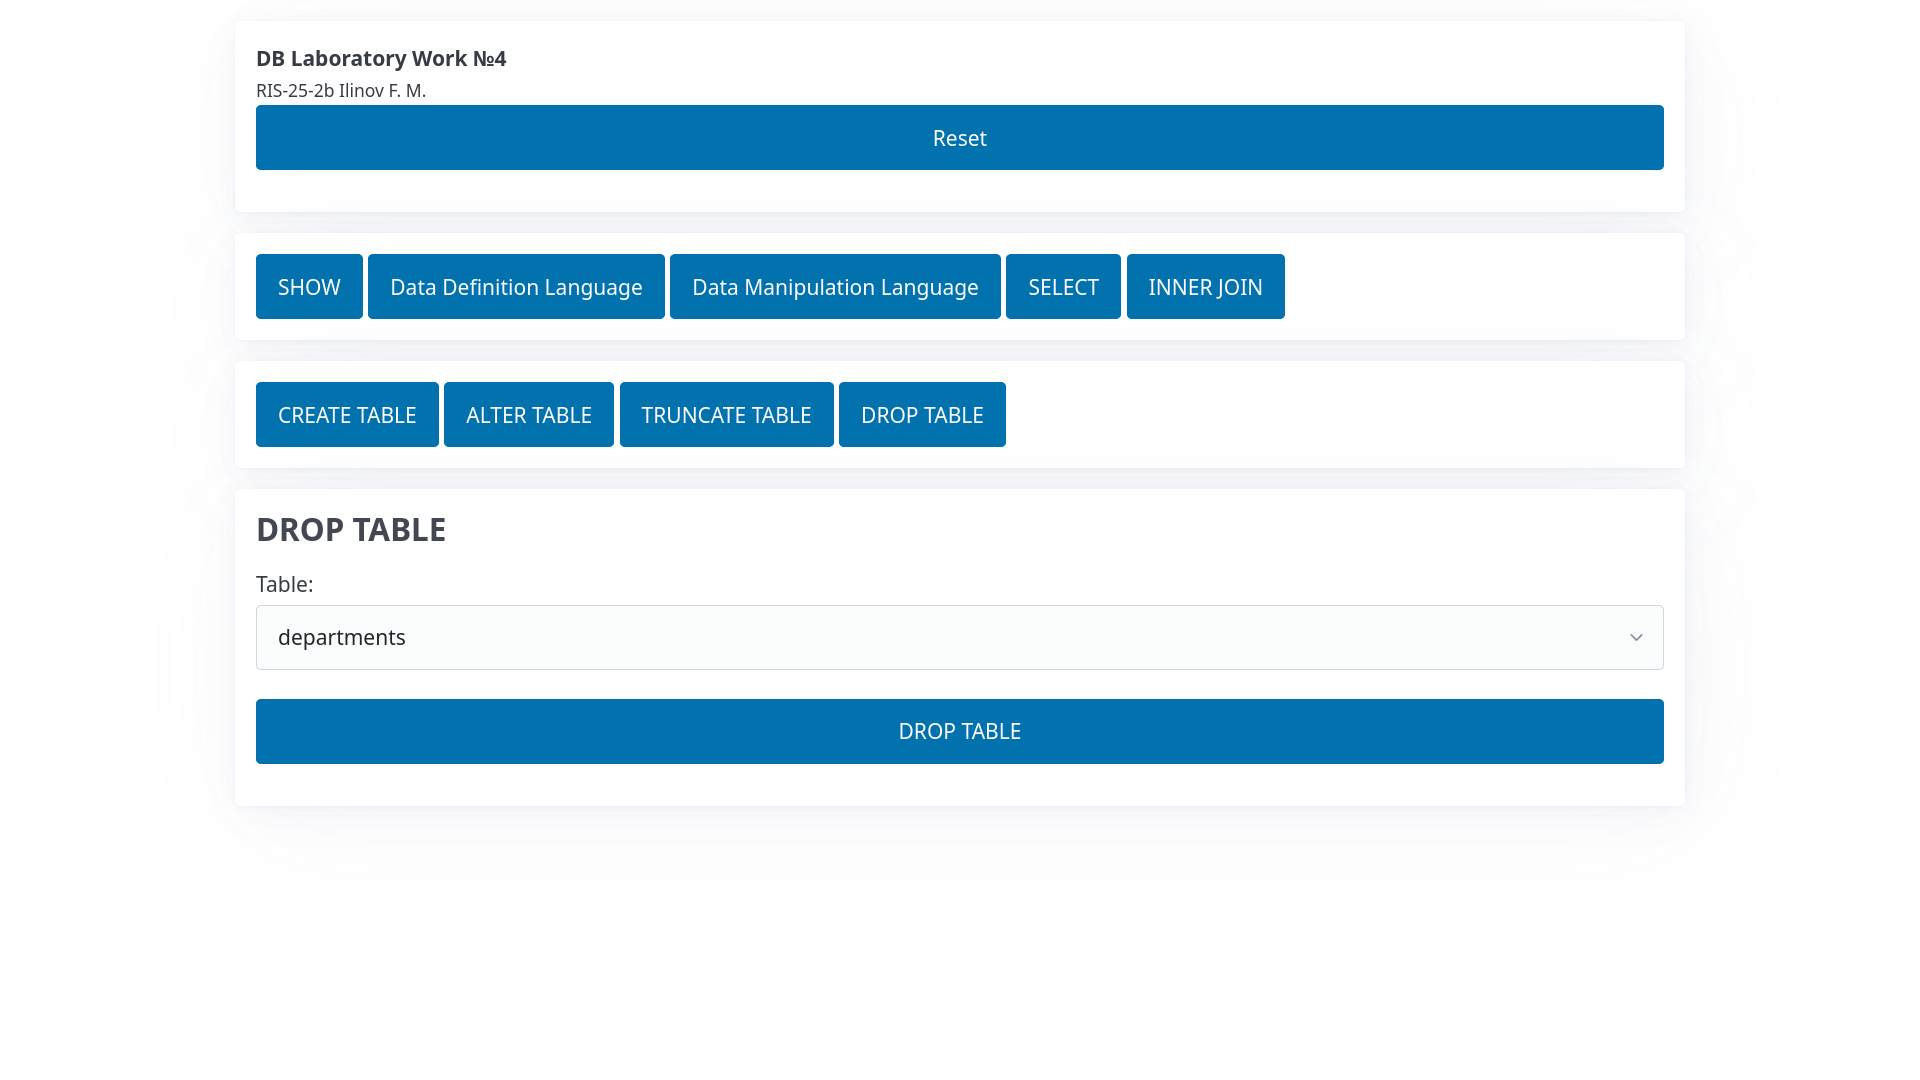
\includegraphics[width=\textwidth]{img_ddl_drop}
    \caption{Удаление сущности оператором DROP TABLE CASCADE}
    \label{fig:fig-ddl-drop}
\end{figure}

Снимок экрана пакетного добавления нескольких кортежей оператором INSERT INTO представлен на рисунке~\ref{fig:fig-dml-insert}.

\begin{figure}[H]
    \centering
    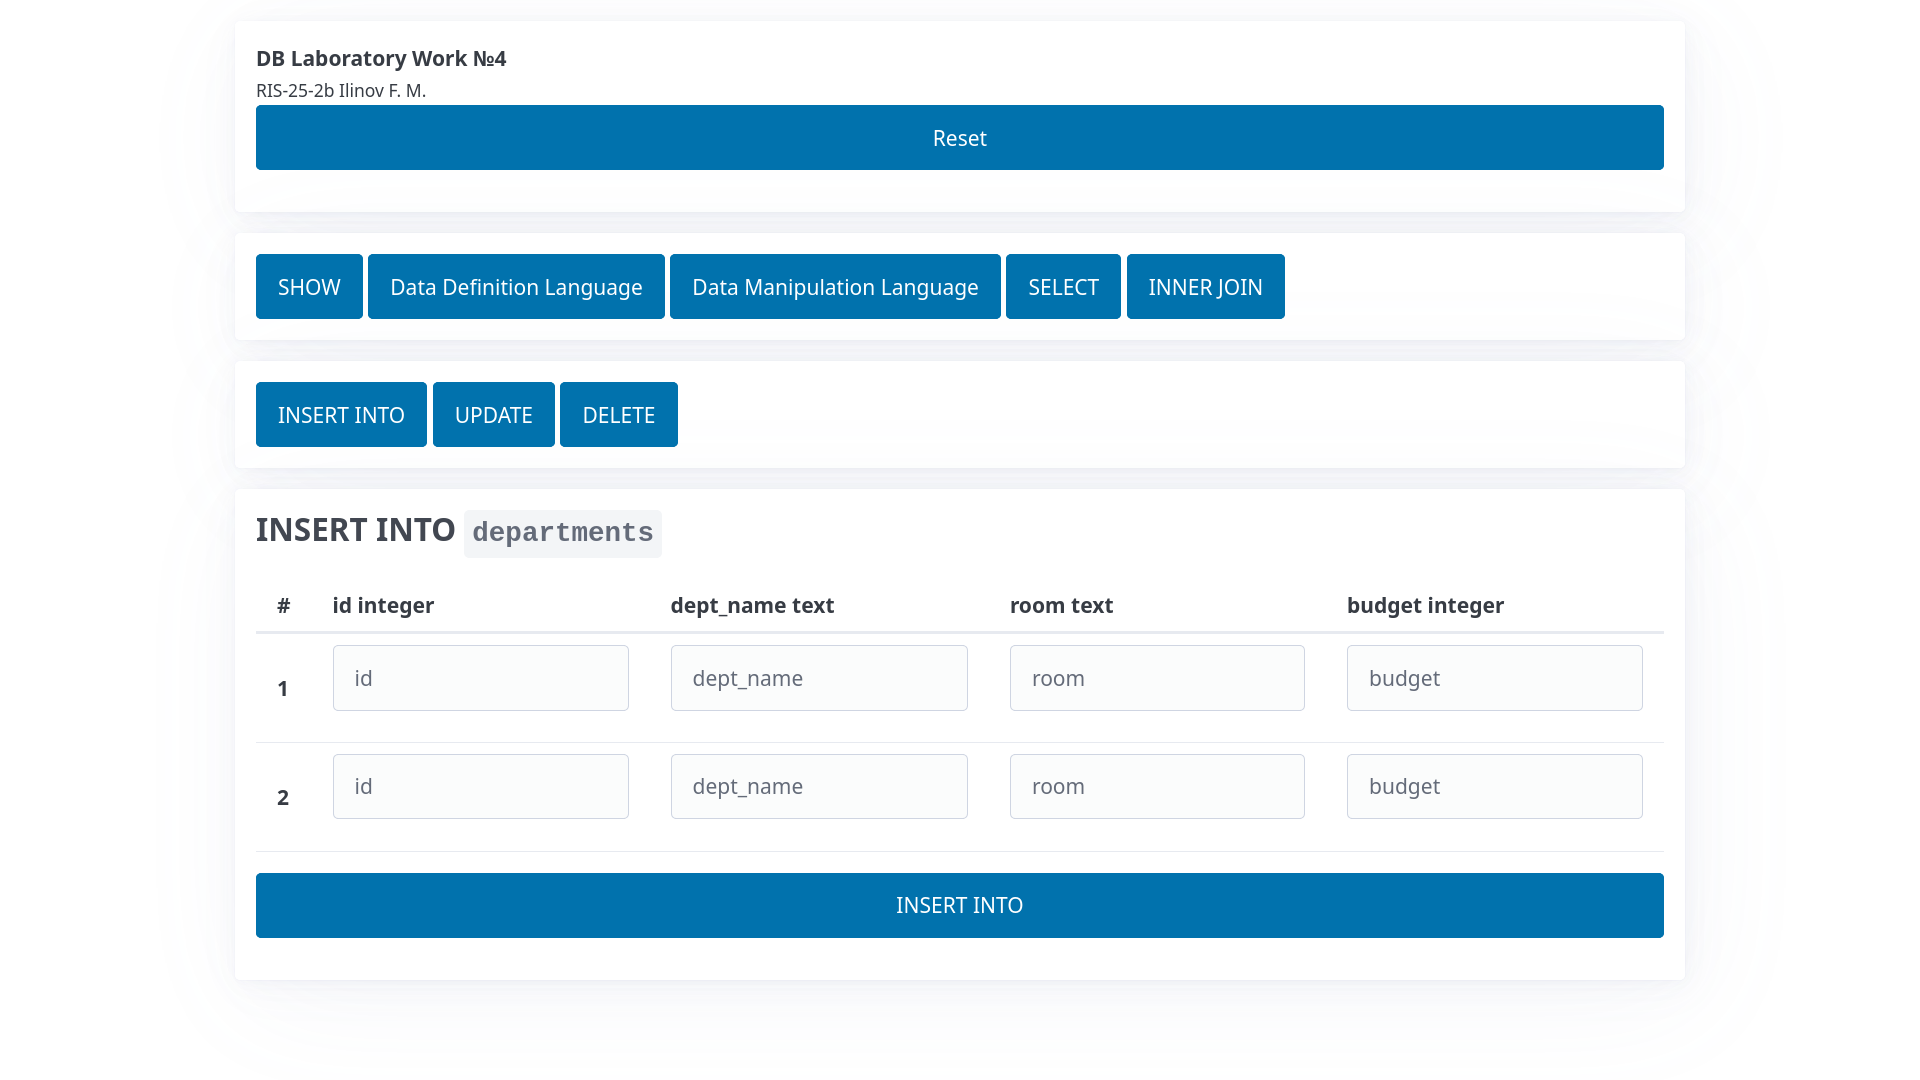
\includegraphics[width=\textwidth]{img_dml_insert}
    \caption{Пакетная вставка записей с помощью команды INSERT INTO}
    \label{fig:fig-dml-insert}
\end{figure}

Снимок экрана изменения данных оператором UPDATE с предикатом WHERE приведен на рисунке~\ref{fig:fig-dml-update}.

\begin{figure}[H]
    \centering
    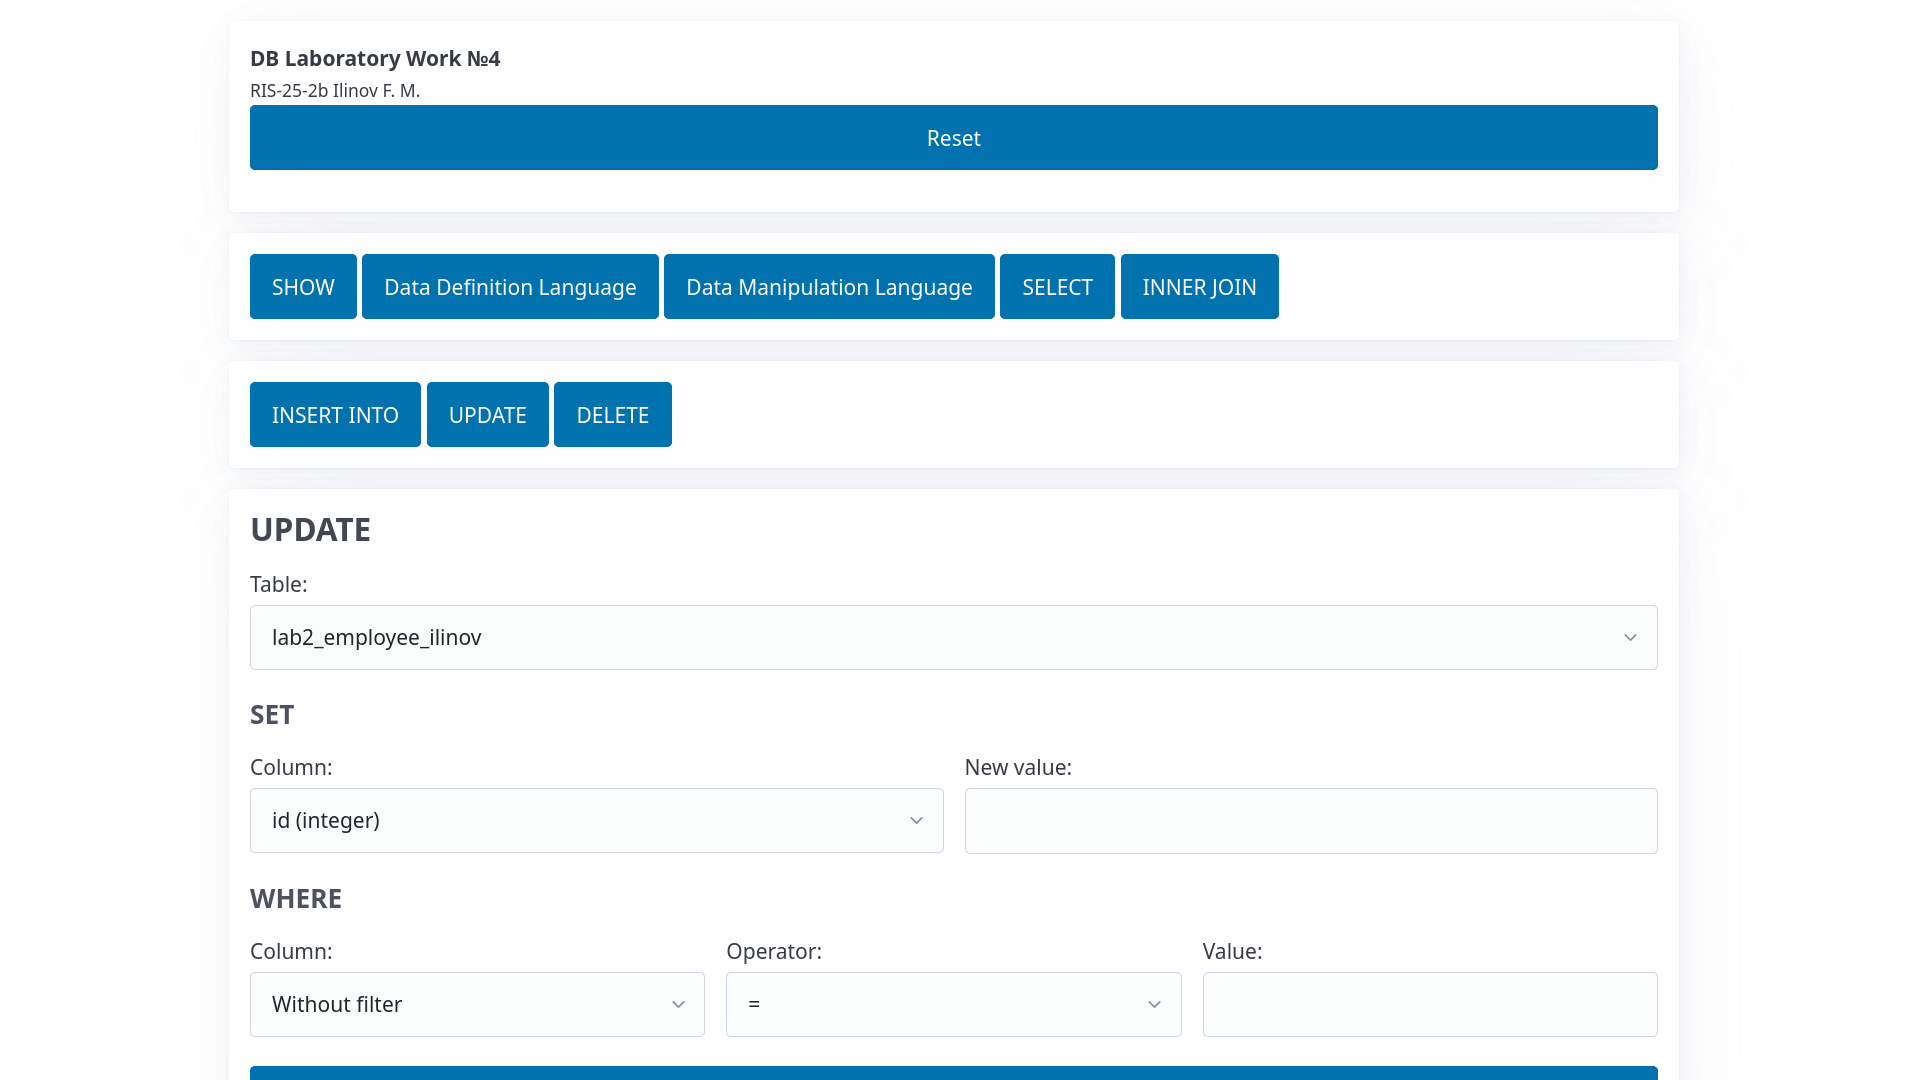
\includegraphics[width=\textwidth]{img_dml_update}
    \caption{Обновление данных с условием фильтрации}
    \label{fig:fig-dml-update}
\end{figure}

Снимок экрана удаления записей оператором DELETE приведен на рисунке~\ref{fig:fig-dml-delete}.

\begin{figure}[H]
    \centering
    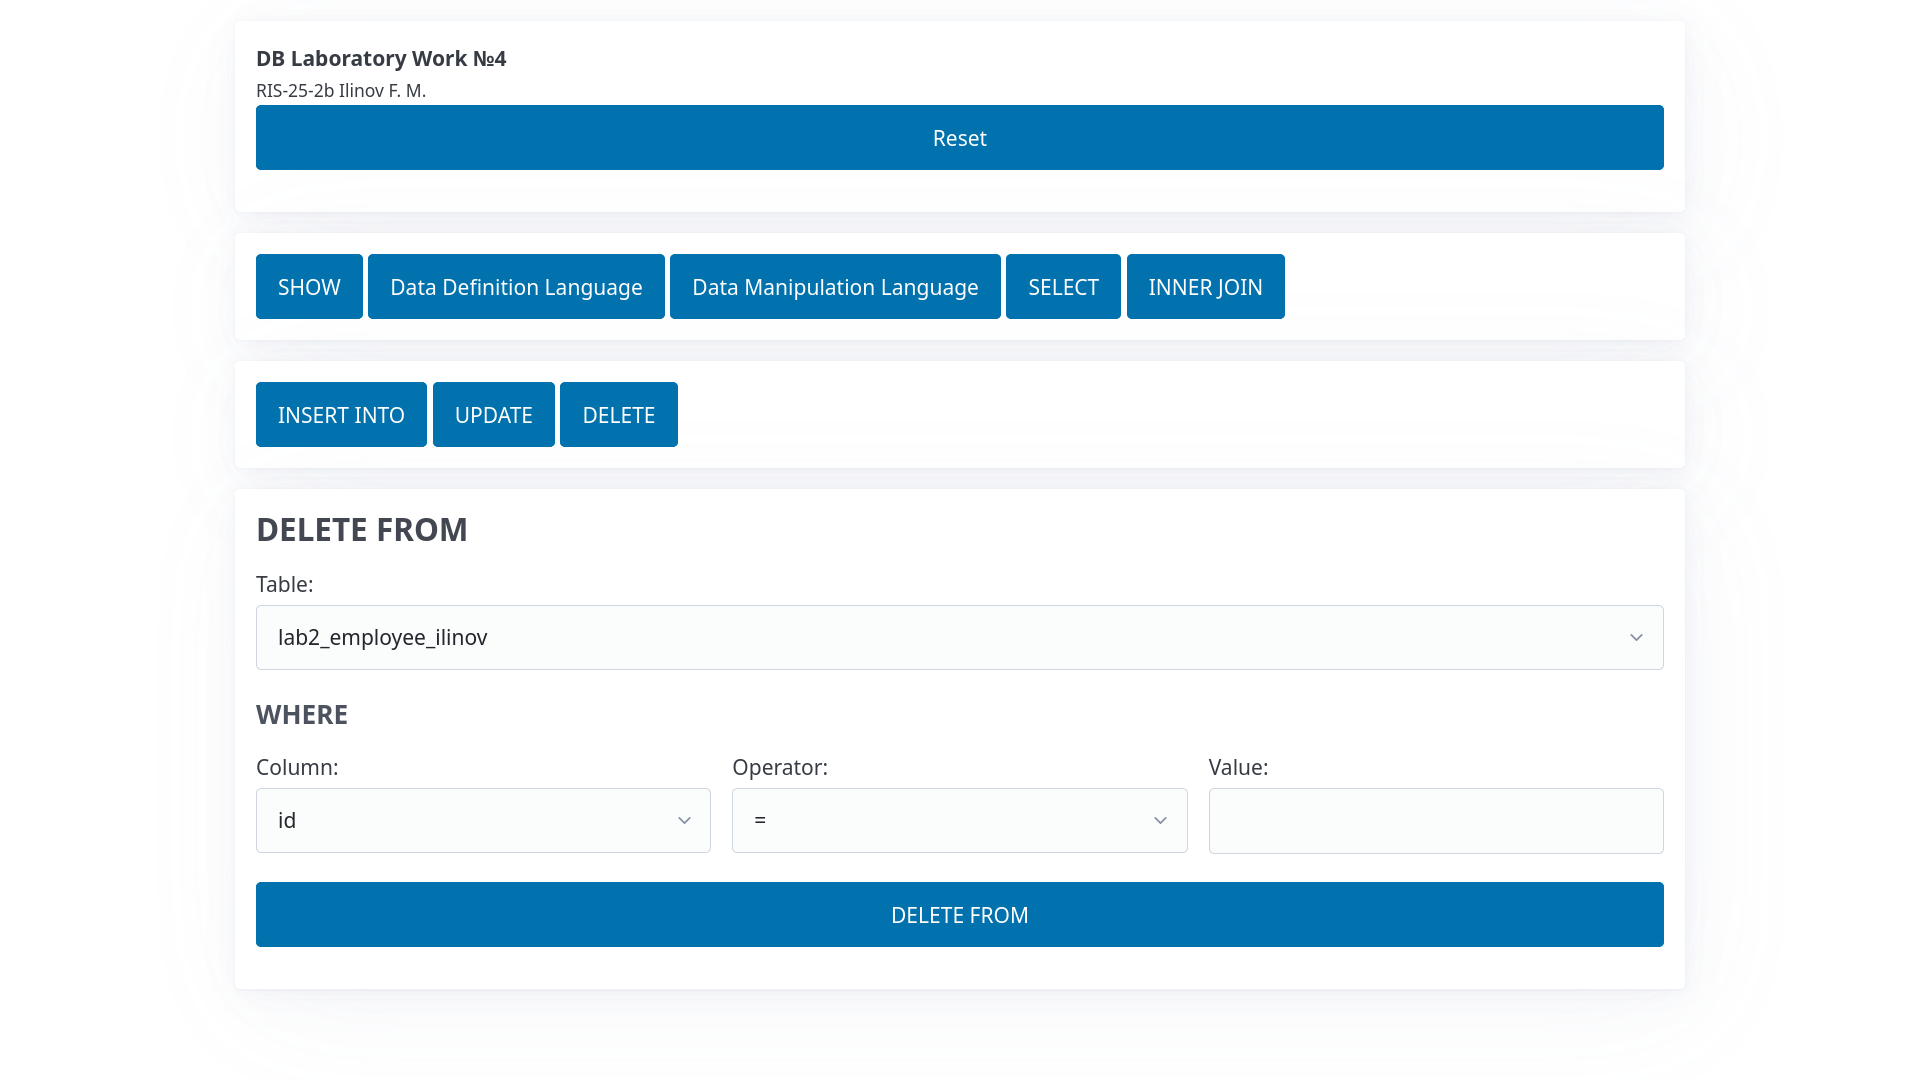
\includegraphics[width=\textwidth]{img_dml_delete}
    \caption{Удаление записей оператором DELETE FROM по условию}
    \label{fig:fig-dml-delete}
\end{figure}

Снимок экрана параметризованной выборки SELECT с фильтрацией и сортировкой приведен на рисунке~\ref{fig:fig-select}.

\begin{figure}[H]
    \centering
    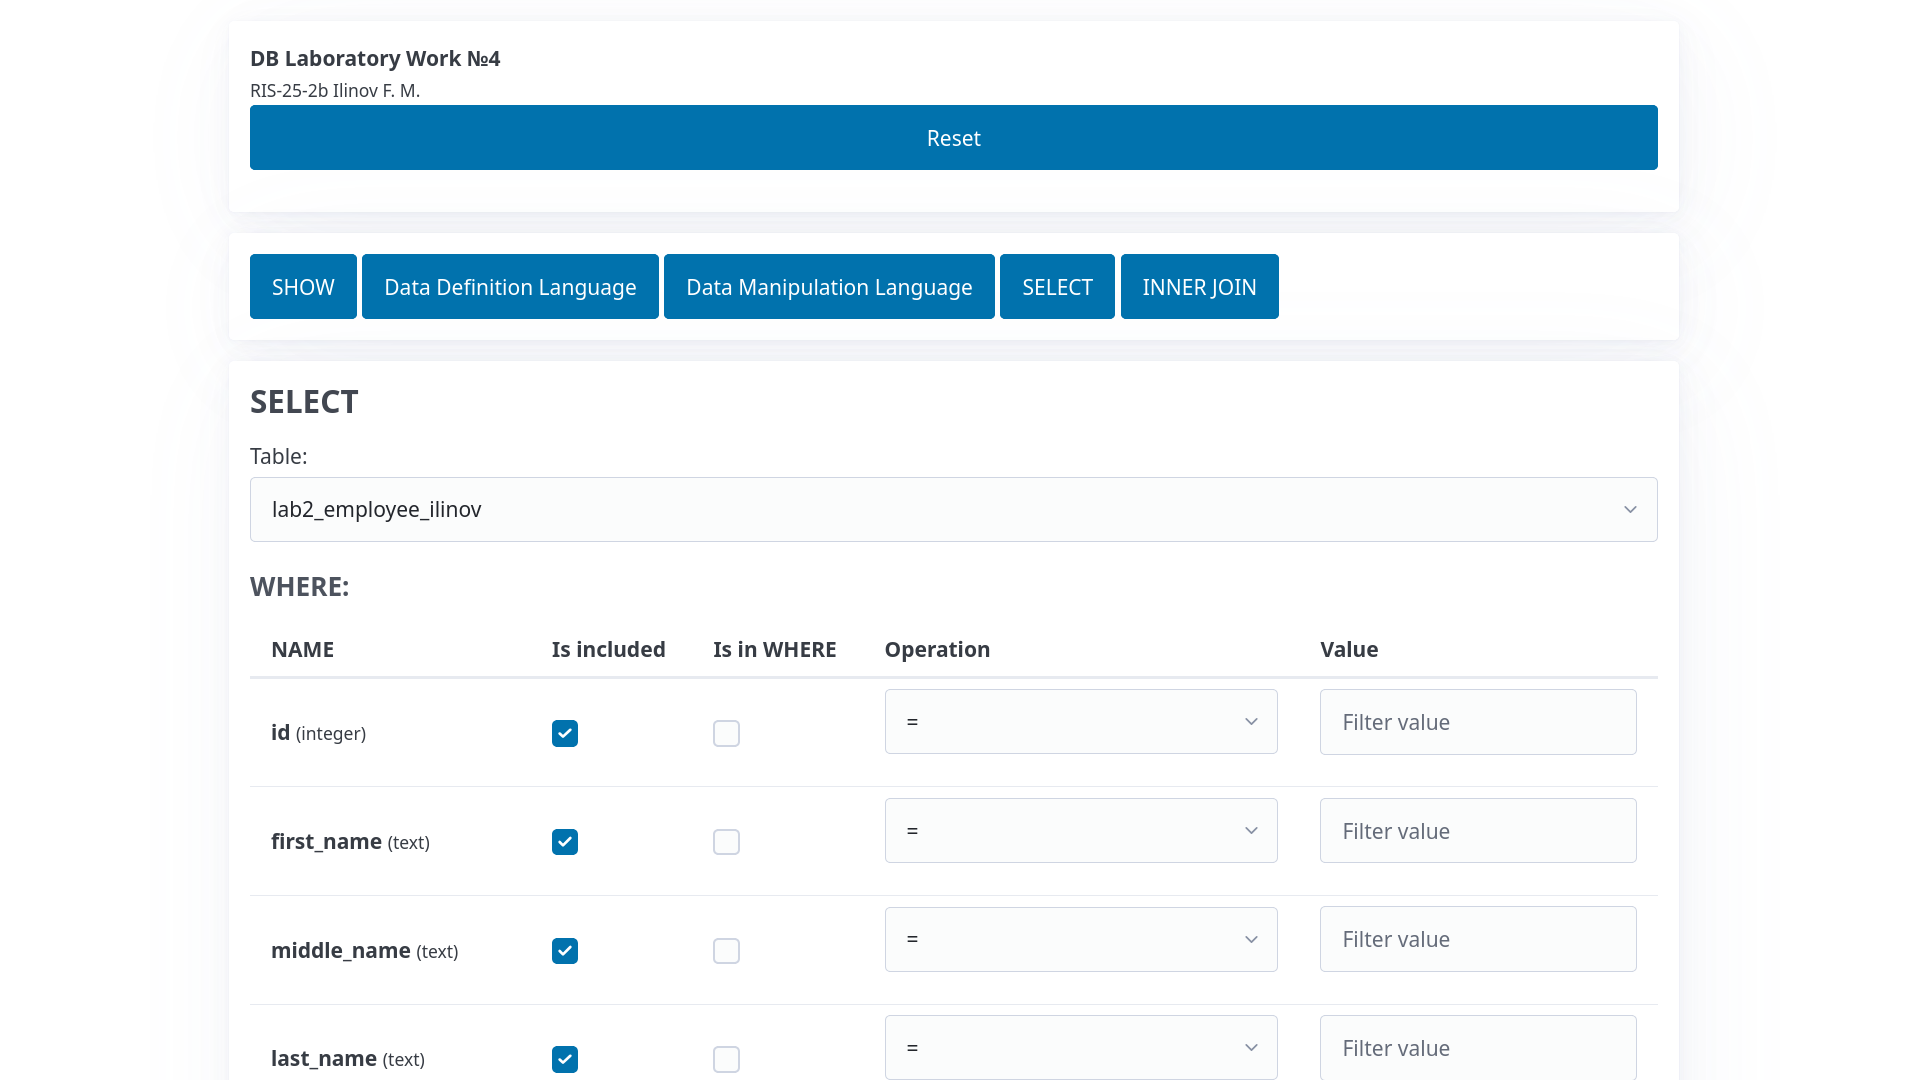
\includegraphics[width=\textwidth]{img_select}
    \caption{Результаты параметризованной выборки SELECT ... WHERE}
    \label{fig:fig-select}
\end{figure}

Снимок экрана внутреннего соединения двух таблиц оператором INNER JOIN представлен на рисунке~\ref{fig:fig-join}.

\begin{figure}[H]
    \centering
    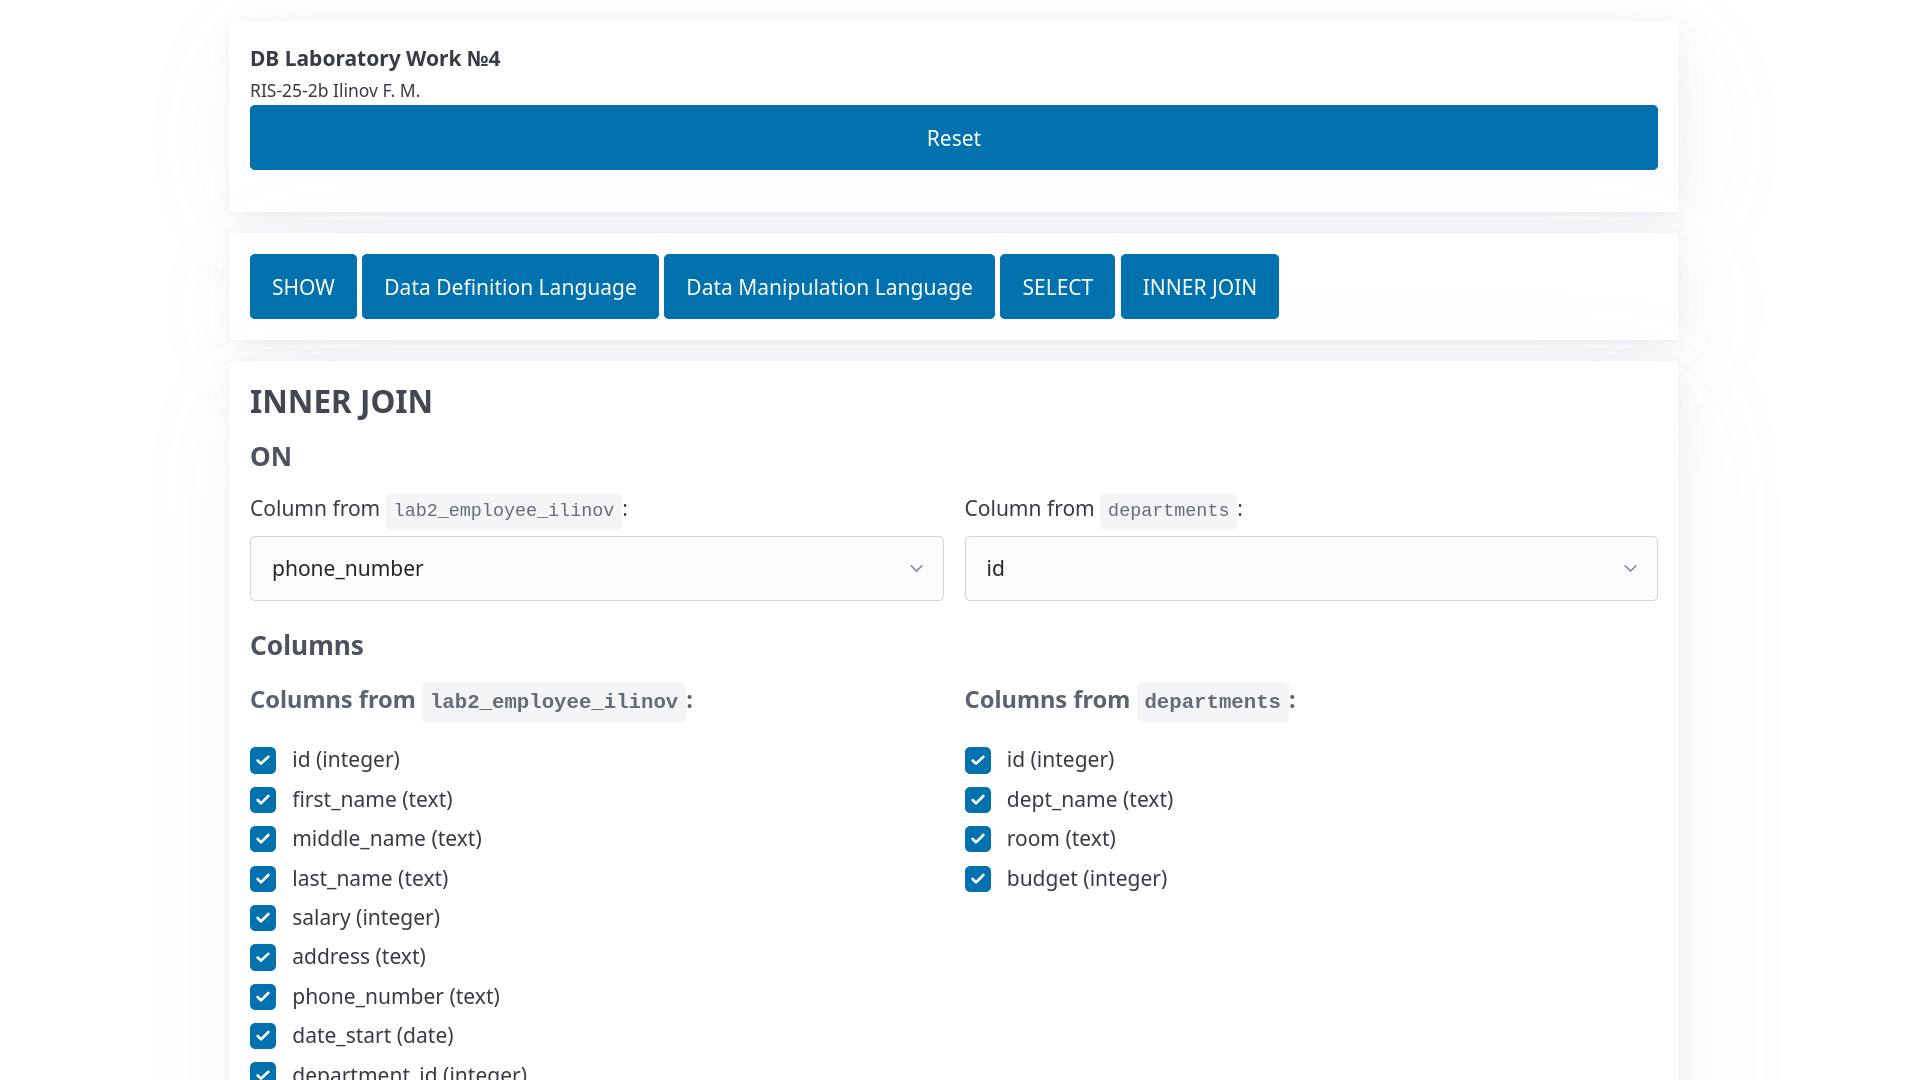
\includegraphics[width=\textwidth]{img_join}
    \caption{Результаты реляционного соединения INNER JOIN ... ON}
    \label{fig:fig-join}
\end{figure}

На всех этапах тестирования сформированные SQL-запросы корректно валидировались и исполнялись СУБД PostgreSQL, а результирующие наборы данных и системные уведомления в полном объеме выводились в веб-интерфейсе.
